\documentclass{standalone}
%outline around text
\usepackage[outline]{contour}
\contourlength{1.3pt}

%tikz
\usepackage{tikz}
\usetikzlibrary{knots, cd, calc}

\begin{document}
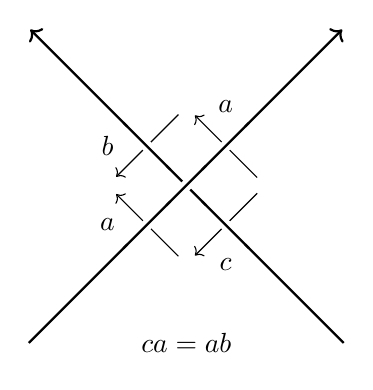
\begin{tikzpicture}
\begin{knot}[clip width = 5]
\strand[black, thick, ->] (0, 0) -- (4, 4);
\strand[black, thick, ->] (4, 0) -- (0, 4);

\strand[black, ->] (1.9, 1.1) -- (1.1, 1.9);
\strand[black, ->] (1.9, 2.9) -- (1.1, 2.1);
\strand[black, ->] (2.9, 2.1) -- (2.1, 2.9);
\strand[black, ->] (2.9, 1.9) -- (2.1, 1.1);

\node at (1, 1.5) {$a$};
\node at (1, 2.5) {$b$};
\node at (2.5, 3) {$a$};
\node at (2.5, 1) {$c$};

\node at (2, 0) {$ca = ab$};
\end{knot}
\end{tikzpicture}
\end{document}